\section{Принцип работы лазера}



\subsection{Скоростные уравнения в лазере}



\textbf{Чертырёхуровневая схема}.
Есть уровни $1,4,3,2$ -- $E_{14} \gg k T$. Также $\tau_{23} = 10$пс. Также с $\tau_{41} = 10$пс. Итого очень легко добиться инверсии населенности между третьим и четвертым уровнем. Накачка происходит с первого на второй уровень. 




\begin{figure}[hb]
    \centering
    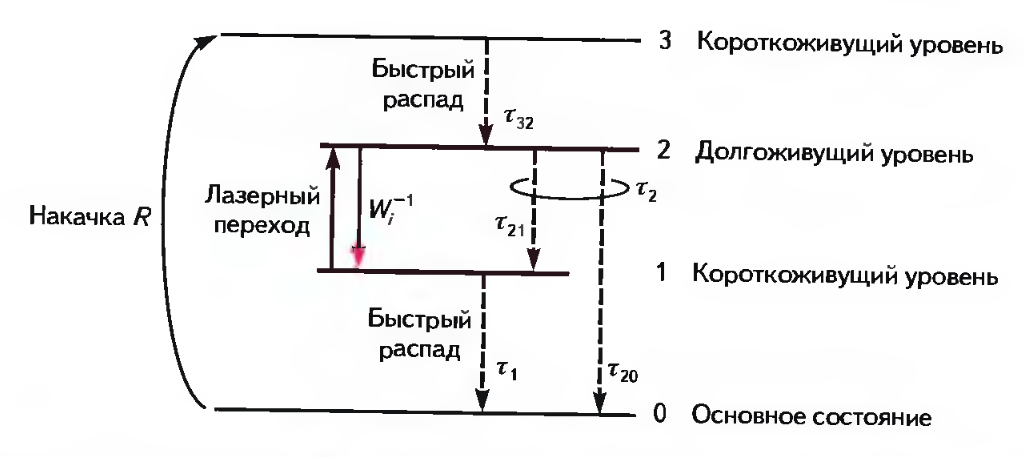
\includegraphics[width=0.45\textwidth]{figures/012.png}
    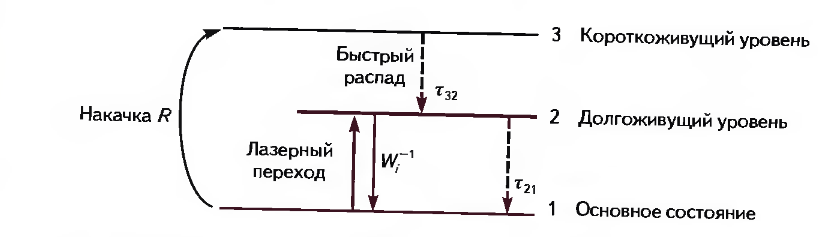
\includegraphics[width=0.45\textwidth]{figures/013.png}
    % \caption{}
    %\label{fig:}
\end{figure}



\textbf{Лазер}.
Есть некоторая среда, есть накачка, с помощью которой происходит переброс с $1$ на $4$ уровень. Пока что это только усилитель. Теперь добавим зеркало 100\% слева и 50\% справа. 

И тут на сцену выходит произвольное излучение. Как только один полетит в удачном направлении, захватит с собой остальных -- лавина, успех. 



\textbf{Моды в лазере}.
Обычно разность частот между двумя последовательными модами $\delta \nu = c/2L$. Например, при $L=1$ м, $\Delta \nu = 150$ МГц. 






\subsection{Эталон фабри-перо как оптический элемент для селекции мод}



Как известно, максимум пропускания эталона Фабри-Перо:
\begin{equation*}
    \nu_n = \frac{n c_0}{2 n_r L_1 \cos \theta'},
\end{equation*}
где $n$ -- целое число, $n_r$ -- показатель преломления, $L_1 \ll L$ -- его длина. И если теперь разность частот $\Delta \nu = c/2L$ окажется больше или равновной $\Delta \nu_c/2$ -- ширины пика пропускания эталона, то эталон отселектирует моду в центре линии от её соседей.

\begin{figure}[htb]
    \centering
    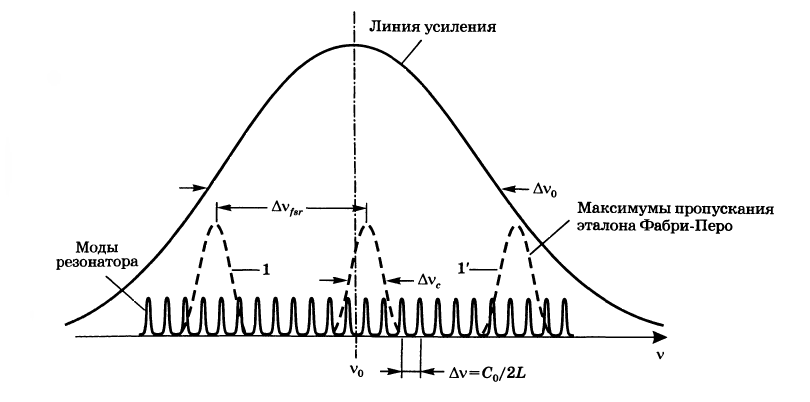
\includegraphics[width=0.5\textwidth]{figures/014.png}
    \caption{Селекция продольных мод с помощью эталона Фабри-Перо, работающего на пропускание}
    %\label{fig:}
\end{figure}








\subsection{Эффект Поккельса}

Рассмотрим \textit{ангармонический осциллятор}  при наличии внешнего постоянного электрического поля $E_0$ 
\begin{equation*}
    \ddot{r} + 2 \gamma \dot{r} + \omega_0^2 r + \beta r^2 = -\frac{e}{m}E_0,
\end{equation*}
где $\beta$ -- постоянная. Считая $r = r_0 + q$ можем перейти к уравнению с новой частотой
\begin{equation*}
    \ddot{q} + 2 \gamma \dot{q} + (\omega_0^2+ 2\beta r_0) q =0,
\end{equation*}
откужа видно изменение частоты колебания на 
\begin{equation*}
    \Delta \omega_0^2 = -\frac{2 e \beta}{m \omega_0^2} E_0^2.
\end{equation*}
Смещение собственных частот меняет кривую дисперсии, т.е. показатель преломления $n$ среды. В простейшем случае, когда $\omega_0$ одна (см. \S 84), изменение $n$ определяется выражением
\begin{equation*}
    \Delta n = \frac{\partial n}{\partial \omega_0^2} \Delta \omega_0^2 = - \frac{\partial n}{\partial \omega_0^2} 
    - \frac{\partial n}{\partial \omega_0^2} \frac{2e\beta}{m \omega_0^2} E_0 = 
    \frac{\partial n}{\partial \omega} \frac{e\beta}{m \omega \omega_0^2} E_0.
\end{equation*}
При фиксированном внешнем $\vc{E}_0$ величина $\Delta n$ зависит от направления распространения света.
Это сказывается на двойном преломлении среды. \textit{Изменеие двойного преломления вещества из-за смещения собственной частоты во внешнем электрическом поле называется электрооптическим эффектом Поккельса}.

В этом эффекте изменения пропорциональны первой степени $E_0$. \textit{Эффект Поккельса может наблюдаться только в 
кристаллах, не обладающих центром симметрии.} Устройство, основанное на эффекте Поккельса, называют \textit{ячейкой Поккельса}. 

Она представляет собой кристалл, помещаемый между двумя скрещенными николями. 
Такое устройство действует так же, как и ячейка Керра. Николи
не пропускают свет, когда нет внешнего электрического поля,
но при наложении такого поля пропускание появляется. 
Необходимо, чтобы кристалл до наложения внешнего электрического
поля не давал двойного преломления. Этого можно достигнуть,
если взять оптически одноосный кристалл, вырезанный 
перпендикулярно к оптической оси, а свет направить вдоль этой оси.
Внешнее поле может быть направлено либо перпендикулярно
(поперечный модулятор света), либо параллельно 
распространению света (продольный модулятор).



\subsection{Модуляция добротности}


Пройдя поляризатор свет поляризуется, а обе компонент испытывают различные фазовые набеги, что приводит к сдвигу фаз:
\begin{equation*}
    \Delta \varphi = k \Delta n\, L',
\end{equation*}
где $k = 2\pi/\lambda$, $\Delta n = n_x - n_y$, а $L'$ -- длина кристалла. При $\Delta \varphi = \pi/2$ волна становится поляризована по кругу. Отражаясь от зеркала и повторно проходя ячейку Поккельса свет становится линейно поляризованным и макисмум $E_x$ соответсвует минимумум $E_y$. Данное состояние соответствует закрытому затвору. 

Открывается затвор снаятием напряжения смещения в ячейке Поккельса -- при этом исчезает двулучепреломление и входящий свет проходит без изменения его поляризации. 

Ячейка Поккельса -- пассивный модулятор добротности. 


